\chapter{TestBeam setup}

\begin{figure}[!ht]
    \centering
    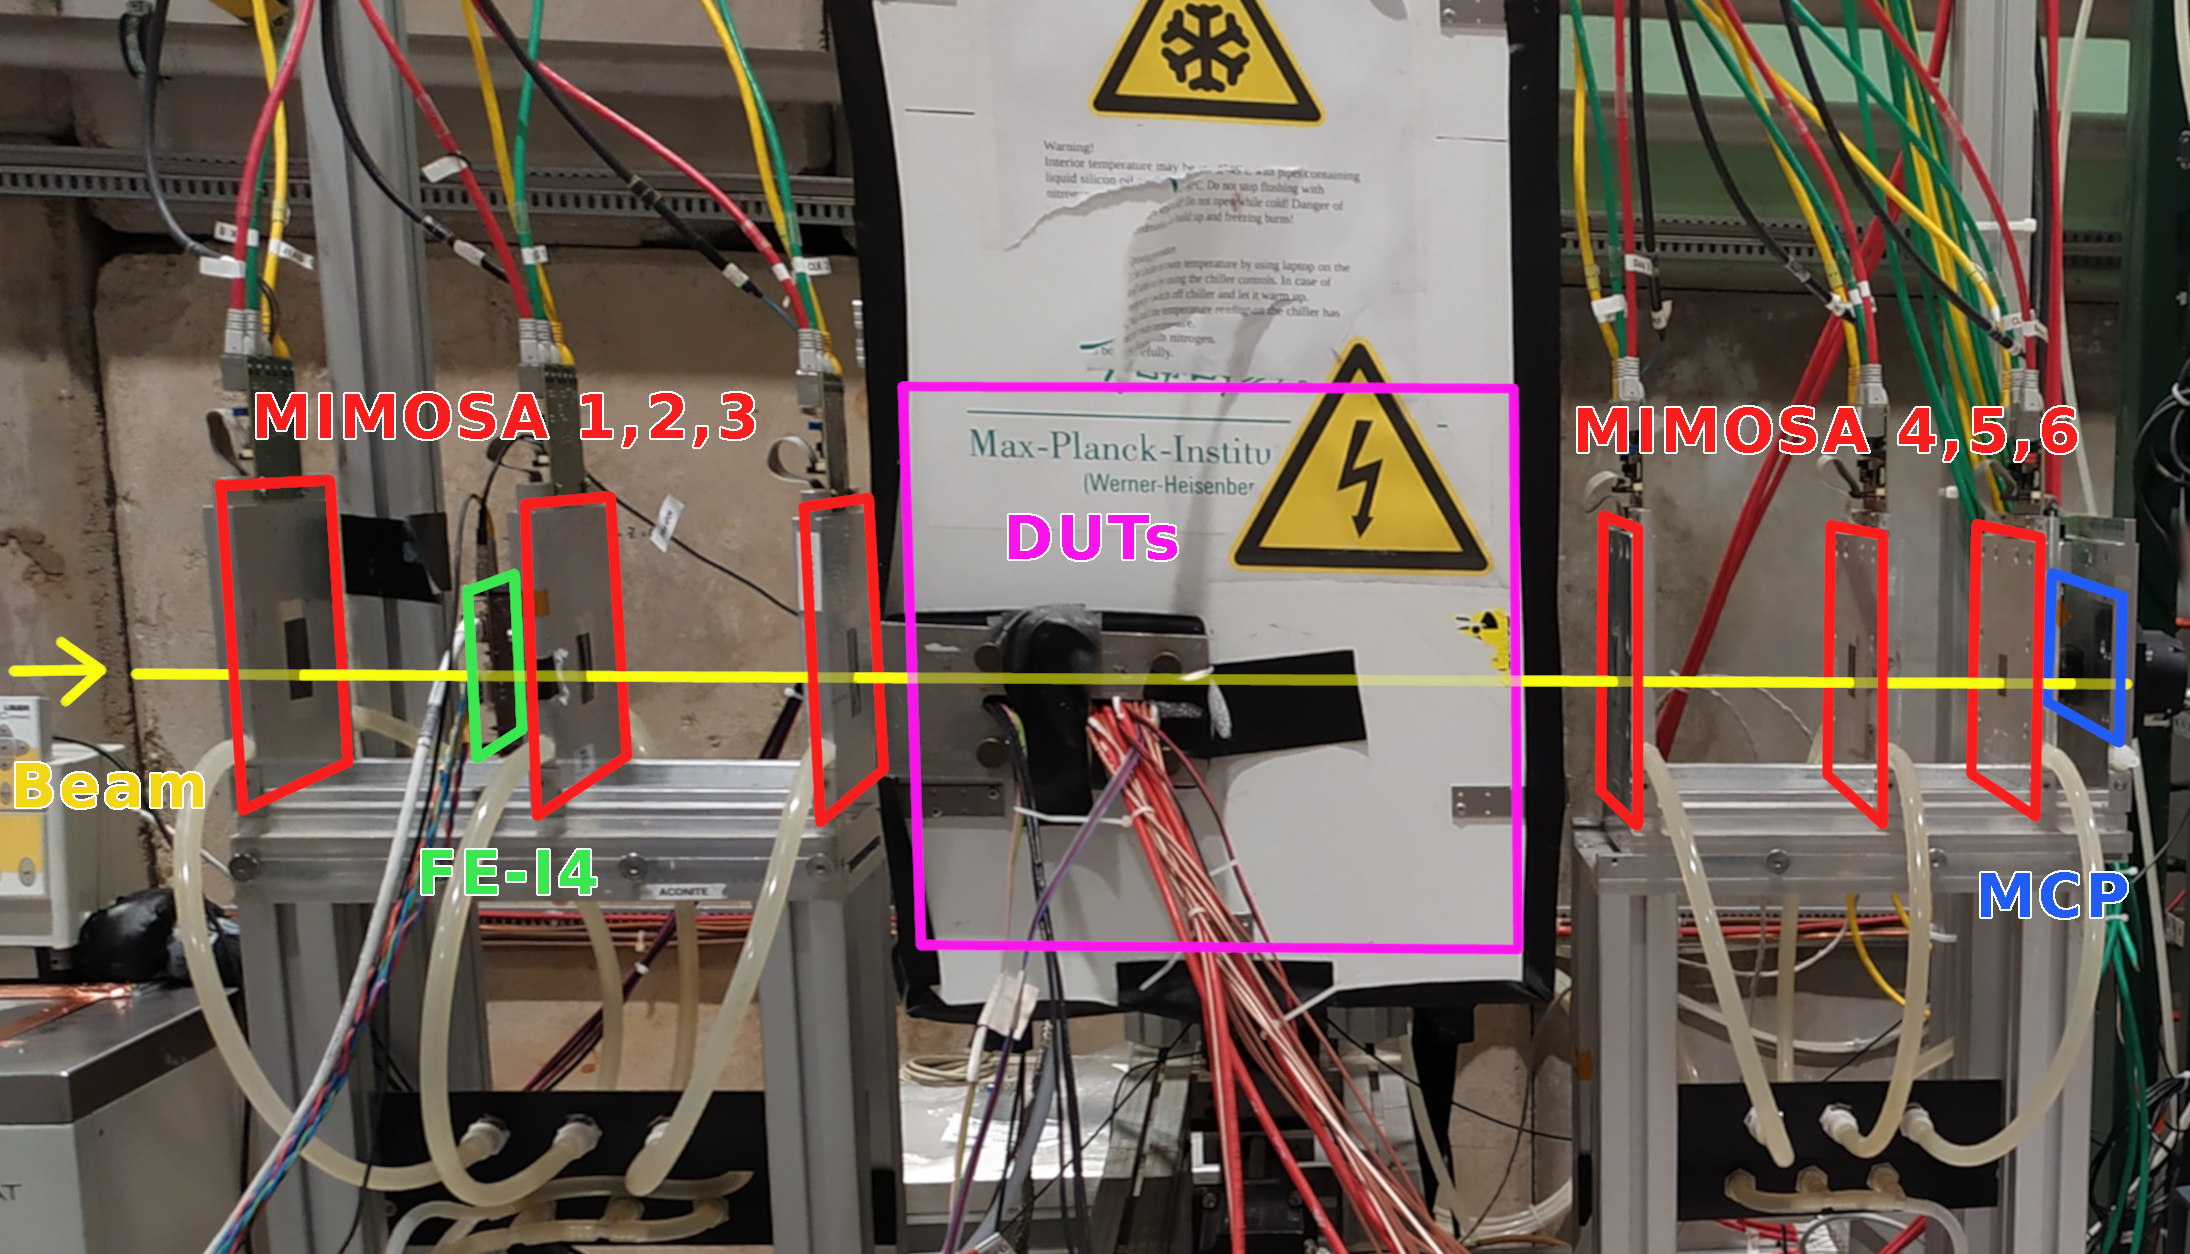
\includegraphics[width=.95\textwidth]{Images/TestBeam_setup/TestBeam_setup_redrawn.png}
    \caption{The components of the TestBeam: six MIMOSA planes, FE-I4, MCP and cooling box containing the DUTs}
    \label{fig:testbeam_setup}
\end{figure}
% description of components:
% • Trigger logic unit for particle passing
% • FEi4 to select a region of interest
% • Mimosa planes for tracking (X and Y position data)
% • MCP for time reference 
% • Cooling box containint the DUTs, (can be tilted with respect to the beam direction)
% • 120 GeV beam of pion
\section{MIMOSA planes}
tracking provide data on the tracks of the particles \marginpar{\flushleft mention how the tracking was done}
defects of the planes

\section{FEi4}
Region of interest, show plots
problems with that \marginpar{\flushleft maybe should be in the appendix}

\section{MCP}\label{sec:MCP_description}
The microchannel plate (MCP) detector consists of a single block of resistive material with an large number of evenly spaced small tubes (microchannels) connecting one face to the other. The main working principle is similar to that of an electron multiplier. When a voltage is applied between the two sides a potential gradient is established along the channels. Whenever a charged particle hits the inner wall of the tubes multiple secondary electrons are emitted, these electrons then are accelerated and hit the opposite wall in the channel, causing the emission of further secondary electrons. As a result, an exponentially increasing number of electrons can be extracted from the output. This detector can provide very fast response time and it was used as a reference for the time resolution of the other devices.

% \begin{figure}
%     \centering
%     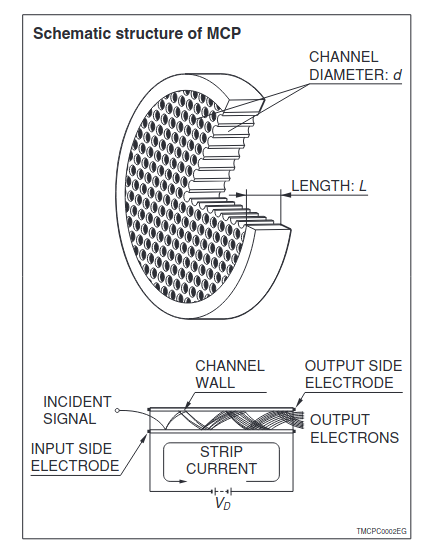
\includegraphics[width=.7\textwidth]{Images/TestBeam_setup/MCP diagram HAMAMATSU.png}
%     \caption{Schematics of an MCP.\\ 
%     Top: structure of the detector with a cross-sectional view of the channels.\\
%     Bottom: illustration of the electron multiplication principle happening inside the channels, which produces the amplified signal}
%     \label{fig:MCP_diagram}
% \end{figure}


\begin{figure}
\begin{minipage}[c]{.45\linewidth}
    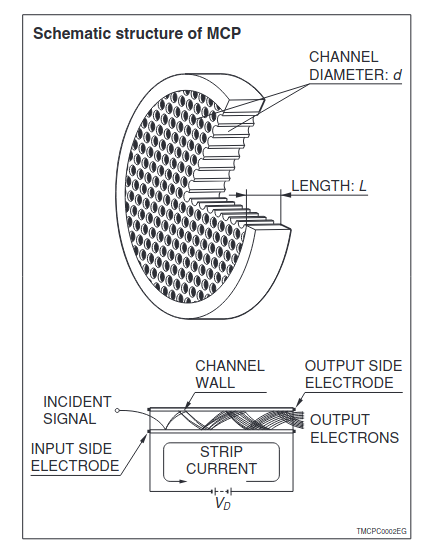
\includegraphics[width=1\linewidth]{Images/TestBeam_setup/MCP diagram HAMAMATSU.png}
\end{minipage}
\hfill
\begin{minipage}[c]{.5\linewidth}
    \caption{
    Schematics of an MCP.\\ 
    Top: structure of the detector with a cross-sectional view of the channels.\\
    Bottom: illustration of the electron multiplication principle happening inside the channels, which produces the amplified signal.}
\end{minipage}
\label{fig:MCP_diagrame}
\end{figure}


\subsection{Time resolution of the MCP}
The time resolution of the MCP was first calculated by comparing the time difference of two independent sensors (CNM-W4 and CNM-W5) and the MCP. In this way, it was possible to build a system of three equations of the time differences. 
\begin{equation}\label{eq:time_res_system_eqs}
    \begin{cases}
        t_{1-2} = t_1 - t_2  \\
        t_{1-MCP} = t_1 - t_{MCP} \\
        t_{2-MCP} = t_2 - t_{MCP} \, .
    \end{cases}
\end{equation}

The time distributions (left sides of the equations) were fitted with a gaussian function, each with a width $\sigma_{ij} = \sigma_i \oplus \sigma_j$, where $i$ and $j$ are two of the devices in Equation \ref{eq:time_res_system_eqs} (i.e. MCP, CNM-W4 and CNM-W5). Assuming that the devices were all independent, their time resolutions would also be independent. This gave a system of three equations with three unknowns, which could be solved analytically to find each individual time resolution: $\sigma_1$, $\sigma_2$, $\sigma_{MCP}$.

The results computed this way are shown in Table \ref{tab:MCP_time_resolution}.
\begin{table}[!ht]
    \begin{center}
        \caption{Time resolution values of the MCP. The "Error" is the statistical uncertainty, since the calculation was repeated for all the available runs.}
        \label{tab:MCP_time_resolution}
        \begin{tabular}{ | c | c | c | c | }
            \hline
            Voltage [$\si{V}$] & 2500 & 2600 & 2800 \\ 
            \hline 
            Time resolution [$\si{ps}$] & 36.52 & 16.48 & 3.73 \\  
            Error [$\si{ps}$] & $\pm$0.81 & $\pm$0.57 & $\pm$1.33 \\
            \hline
        \end{tabular}
    \end{center}
\end{table}


\section{Oscilloscopes}
The signal generated by the DUT was recorded by two four-channel oscilloscopes: channel 1 (denoted as Ch1) of both oscilloscopes was connected to the MCP (which was used as time reference, described previously in Section \ref{sec:MCP_description}). So, up to 6 channels were available in each batch to be attached to the DUTs.

